\documentclass[10pt, a4paper]{scrartcl}

% --- Language & Encoding ---
\usepackage[utf8]{inputenc}
\usepackage[T1]{fontenc}
\usepackage{lmodern}
\usepackage{microtype}

% --- Page Geometry ---
\usepackage[margin=1.5cm, top=1.5cm, bottom=1.5cm, headheight=0cm, headsep=0cm]{geometry}

% --- Color Palette (Custom 4-Color Theme) ---
\usepackage[table]{xcolor}
\definecolor{primary}{HTML}{1E3A8A}      % Deep Royal Navy
\definecolor{secondary}{HTML}{0D9488}    % Elegant Teal
\definecolor{darktext}{HTML}{1F2937}     % Charcoal Text
\definecolor{lightbg}{HTML}{F8FAFC}      % Soft Cool Grey/Blue
\definecolor{boxborder}{HTML}{CBD5E1}    % Border Grey
\definecolor{accentbg}{HTML}{F0FDFA}     % Light Teal Tint

% --- Typography & KOMA-Script Customization ---
\addtokomafont{section}{\color{primary}\sffamily\Large\bfseries}
\addtokomafont{subsection}{\color{secondary}\sffamily\large\bfseries}
\addtokomafont{subsubsection}{\color{darktext}\sffamily\normalsize\bfseries}

% --- Core Packages ---
\usepackage{amsmath, amssymb, amsfonts}
\usepackage{booktabs}
\usepackage{tabularx}
\usepackage{enumitem}
\usepackage{multicol}
\usepackage{caption}
\usepackage{fontawesome5}

% --- Visual Containers & TikZ ---
\usepackage{tcolorbox}
\tcbuselibrary{skins, breakable}

\usepackage{tikz}
\usetikzlibrary{positioning, calc, shapes.geometric, backgrounds, patterns}

% --- Hyperlinks ---
\usepackage[hidelinks, colorlinks=true, linkcolor=primary, citecolor=secondary, urlcolor=secondary]{hyperref}

% --- Paragraph & Spacing Adjustments ---
\setlength{\parindent}{0pt}
\setlength{\parskip}{0.45em}
\setlength{\columnsep}{0.6cm}

% Caption styling
\captionsetup{font={small,sf},labelfont={bf,color=primary},skip=4pt}

% --- Header Banner & Poster Companion Header ---
\newcommand{\posterheader}{%
  \begin{tcolorbox}[
    enhanced,
    colback=primary,
    colframe=primary,
    arc=3mm,
    boxrule=0pt,
    left=12pt, right=12pt, top=12pt, bottom=12pt,
    coltext=white
  ]
    \begin{minipage}[t]{0.68\textwidth}
      {\sffamily\bfseries\tiny\color{accentbg}\MakeUppercase{\faGraduationCap\ 15th European Conference on Autonomous Systems and Neural Robotics (ECASN 2026)}} \par \vspace{4pt}
      {\sffamily\bfseries\Large Adaptive Latent Dynamics for Online Motion Planning in Deformable Robotic Manipulation} \par \vspace{6pt}
      {\small\sffamily \textbf{Elena Rostova}$^{1}$, \textbf{Marcus Vance}$^{1}$, and \textbf{Julian Sterling}$^{2}$} \par \vspace{3pt}
      {\tiny\sffamily $^{1}$Nexa AI Research Institute, Zurich, Switzerland \quad $^{2}$Synapse Autonomous Robotics Lab, Munich, Germany}
    \end{minipage}%
    \hfill
    \begin{minipage}[t]{0.28\textwidth}
      \raggedleft
      \begin{tcolorbox}[
        colback=white,
        colframe=secondary,
        arc=2.5mm,
        boxrule=1.2pt,
        left=6pt, right=6pt, top=6pt, bottom=6pt,
        coltext=darktext
      ]
        \centering
        {\sffamily\bfseries\tiny \color{secondary}\MakeUppercase{Poster Session Companion}} \par \vspace{2pt}
        {\sffamily\bfseries\scriptsize Track: Neural Control} \par \vspace{1pt}
        {\sffamily\bfseries\Large \color{primary} Board \#B-14} \par \vspace{3pt}
        {\tiny\sffamily \faLink\ github.com/nexa-ai/ald-planner}
      \end{tcolorbox}
    \end{minipage}
  \end{tcolorbox}
}

\begin{document}

\posterheader

\vspace{-2pt}

% --- Executive Summary & Poster Highlights Callout ---
\begin{tcolorbox}[
  enhanced,
  colback=accentbg,
  colframe=secondary,
  arc=2mm,
  boxrule=0.8pt,
  left=10pt, right=10pt, top=7pt, bottom=7pt
]
  \begin{multicols}{2}
    {\sffamily\bfseries\small \color{secondary} \faInfoCircle\ EXTENDED ABSTRACT OVERVIEW} \par \vspace{2pt}
    \small This extended abstract serves as the self-contained mathematical and empirical companion to Poster \#B-14 at ECASN 2026. We investigate real-time trajectory optimization for highly non-linear deformable objects (ropes, textiles, elastomers) without relying on fine-tuned physical simulators.
    \columnbreak
    {\sffamily\bfseries\small \color{secondary} \faCheck\ KEY NOVEL CONTRIBUTIONS} \par \vspace{2pt}
    \begin{itemize}[leftmargin=12pt, topsep=1pt, itemsep=1pt, parsep=0pt]
      \item \textbf{Latent Manifold Encoding}: Self-supervised variational encoder mapping raw point clouds to low-dimensional linear state spaces.
      \item \textbf{Adaptive Model Filter}: Recursive least-squares update yielding sub-12ms re-planning latency under unmodelled elastic deformations.
    \end{itemize}
  \end{multicols}
\end{tcolorbox}

\vspace{-2pt}

\begin{multicols}{2}

\section{Introduction \& Motivation}
Deformable object manipulation (DOM) represents a foundational bottleneck in industrial automation and surgical robotics. Unlike rigid bodies whose kinematics are fully parameterized by six degrees of freedom ($SE(3)$), deformable materials like silicone cables, soft biological tissues, and garments exhibit infinite-dimensional configuration spaces \cite{sterling2024}. 

Existing solutions generally fall into two extremes:
\begin{enumerate}[leftmargin=14pt, itemsep=1pt, topsep=2pt]
  \item \textbf{Finite Element Models (FEM)}: Highly accurate but computationally prohibitive for real-time model-predictive control (MPC).
  \item \textbf{Model-Free Reinforcement Learning}: Highly adaptable but sample-inefficient and vulnerable to distribution shifts in material elasticity.
\end{enumerate}

To bridge this gap, we present \textbf{Adaptive Latent Dynamics (ALD)}, a hybrid paradigm uniting low-dimensional visual representation learning with real-time adaptive linear state-space identification.

\begin{center}
  \begin{tcolorbox}[
    colback=lightbg,
    colframe=boxborder,
    arc=2mm,
    boxrule=0.6pt,
    left=4pt, right=4pt, top=6pt, bottom=4pt
  ]
    \centering
    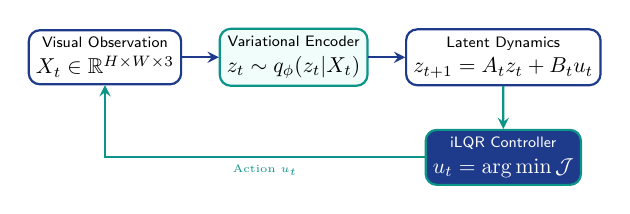
\begin{tikzpicture}[scale=0.78, every node/.style={transform shape}]
      % Nodes
      \node[draw=primary, fill=white, rounded corners=4pt, thick, minimum width=2.1cm, minimum height=0.85cm, align=center] (obs) {\sffamily\scriptsize Visual Observation\\$X_t \in \mathbb{R}^{H \times W \times 3}$};
      \node[draw=secondary, fill=accentbg, rounded corners=4pt, thick, minimum width=2.0cm, minimum height=0.85cm, align=center, right=0.6cm of obs] (enc) {\sffamily\scriptsize Variational Encoder\\$z_t \sim q_\phi(z_t | X_t)$};
      \node[draw=primary, fill=white, rounded corners=4pt, thick, minimum width=2.0cm, minimum height=0.85cm, align=center, right=0.6cm of enc] (dyn) {\sffamily\scriptsize Latent Dynamics\\$z_{t+1} = A_t z_t + B_t u_t$};
      \node[draw=secondary, fill=primary, text=white, rounded corners=4pt, thick, minimum width=2.1cm, minimum height=0.85cm, align=center, below=0.7cm of dyn] (mpc) {\sffamily\scriptsize iLQR Controller\\$u_t = \arg\min \mathcal{J}$};
      
      % Connections
      \draw[->, >=stealth, thick, color=primary] (obs) -- (enc);
      \draw[->, >=stealth, thick, color=primary] (enc) -- (dyn);
      \draw[->, >=stealth, thick, color=secondary] (dyn) -- (mpc);
      \draw[->, >=stealth, thick, color=secondary] (mpc) -| (obs) node[pos=0.25, below] {\tiny Action $u_t$};
    \end{tikzpicture}
    \captionof{figure}{\sffamily Closed-loop architecture of the ALD control framework.}
    \label{fig:pipeline}
  \end{tcolorbox}
\end{center}

\section{Problem Formulation}
Let $\mathcal{C}$ denote the continuous configuration space of a deformable body driven by robotic end-effector inputs $u_t \in \mathbb{R}^m$. The unknown ground-truth system dynamics governed by physical parameters $\theta^*$ follow:
\begin{equation}
  s_{t+1} = f(s_t, u_t; \theta^*) + w_t, \quad s_t \in \mathcal{C}, \; w_t \sim \mathcal{N}(0, \Sigma_w)
\end{equation}

Because full state $s_t$ cannot be directly measured, we project high-dimensional point clouds $X_t \in \mathbb{R}^{N \times 3}$ into a latent representation $z_t \in \mathbb{R}^d$ ($d \ll N$). We enforce that local latent transitions adhere to a time-varying linear dynamical system:
\begin{equation}
  z_{t+1} \approx A_t z_t + B_t u_t + c_t
\end{equation}
where $A_t \in \mathbb{R}^{d \times d}$, $B_t \in \mathbb{R}^{d \times m}$, and $c_t \in \mathbb{R}^d$ are updated online using an Extended Recursive Least-Squares (eRLS) gain scheme.

\section{Methodology}

\subsection{Variational Latent Space Mapping}
We construct a spatial autoencoder initialized offline using synthetic physics rollouts generated by Vertex Engine. The encoder $q_\phi(z_t | X_t)$ and decoder $p_\psi(X_t | z_t)$ are trained jointly with a temporal consistency term:
\begin{equation}
  \mathcal{L}_{\text{train}}(\phi, \psi) = \mathcal{L}_{\text{recon}} + \beta \mathcal{D}_{\text{KL}} + \lambda \mathbb{E} \left[ \| z_{t+1} - g_\theta(z_t, u_t) \|^2_2 \right]
\end{equation}
where $g_\theta$ represents a global neural prior network.

\subsection{Online Recursive Model Update}
During execution, local system parameters $\hat{\Theta}_t = [A_t, B_t, c_t]$ are estimated at 100\,Hz using real-time observations:
\begin{equation}
  \hat{\Theta}_t = \hat{\Theta}_{t-1} + K_t \left( z_t - \hat{\Theta}_{t-1} \xi_{t-1} \right)^T
\end{equation}
where $\xi_{t-1} = [z_{t-1}^T, u_{t-1}^T, 1]^T$ and $K_t$ is the covariance update matrix incorporating a variable forgetting factor $\gamma_t \in [0.92, 0.98]$.

\columnbreak

\section{Experimental Results}
We benchmarked ALD on a dual-arm Franka Emika Research platform in the Meridian Robotics Laboratory across three representative deformable manipulation tasks.

\begin{center}
  \begin{tcolorbox}[
    colback=lightbg,
    colframe=boxborder,
    arc=2mm,
    boxrule=0.6pt,
    left=4pt, right=4pt, top=6pt, bottom=4pt
  ]
    \centering
    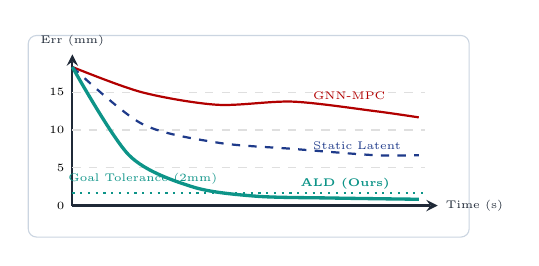
\begin{tikzpicture}[scale=0.80, every node/.style={transform shape}]
      % Graph background
      \draw[fill=white, draw=boxborder, rounded corners=3pt] (0,0) rectangle (7.0,3.2);
      
      % Axes
      \draw[->, >=stealth, thick, color=darktext] (0.7,0.5) -- (6.5,0.5) node[right] {\tiny Time (s)};
      \draw[->, >=stealth, thick, color=darktext] (0.7,0.5) -- (0.7,2.9) node[above] {\tiny Err (mm)};
      
      % Grid lines
      \draw[gray!25, dashed] (0.7,1.1) -- (6.3,1.1);
      \draw[gray!25, dashed] (0.7,1.7) -- (6.3,1.7);
      \draw[gray!25, dashed] (0.7,2.3) -- (6.3,2.3);
      
      % Y-axis labels
      \node[left] at (0.7, 0.5) {\tiny 0};
      \node[left] at (0.7, 1.1) {\tiny 5};
      \node[left] at (0.7, 1.7) {\tiny 10};
      \node[left] at (0.7, 2.3) {\tiny 15};
      
      % Curves
      % Baseline GNN
      \draw[thick, color=red!70!black, smooth] plot coordinates {(0.7,2.7) (1.8,2.3) (3.0,2.1) (4.2,2.15) (5.5,2.0) (6.2,1.9)};
      \node[color=red!70!black, right] at (4.4, 2.25) {\tiny GNN-MPC};
      
      % Static Latent
      \draw[thick, color=primary, smooth, dashed] plot coordinates {(0.7,2.7) (1.8,1.8) (3.0,1.5) (4.2,1.4) (5.5,1.3) (6.2,1.3)};
      \node[color=primary, right] at (4.4, 1.45) {\tiny Static Latent};
      
      % Ours (ALD)
      \draw[very thick, color=secondary, smooth] plot coordinates {(0.7,2.7) (1.6,1.3) (2.6,0.8) (3.6,0.65) (4.8,0.62) (6.2,0.6)};
      \node[color=secondary, right] at (4.2, 0.85) {\tiny \textbf{ALD (Ours)}};
      
      % Target Threshold
      \draw[secondary, dotted, thick] (0.7,0.7) -- (6.3,0.7) node[pos=0.2, above] {\tiny Goal Tolerance (2mm)};
    \end{tikzpicture}
    \captionof{figure}{\sffamily Deformable tracking error over time during dynamic cable routing.}
    \label{fig:results_chart}
  \end{tcolorbox}
\end{center}

\subsection{Benchmark Evaluation Tasks}
\begin{enumerate}[leftmargin=14pt, label=\bfseries T\arabic*., itemsep=1pt]
  \item \textbf{Cable Routing}: Threading a flexible silicone cable through 4 post obstacles.
  \item \textbf{Textile Folding}: Dual-gripper folding of cotton fabrics along specified fold lines.
  \item \textbf{Elastomer Sealing}: Inserting a soft rubber gasket into a curved channel.
\end{enumerate}

\subsection{Quantitative Comparison}
Table~\ref{tab:results} summarizes performance across 50 trials per task against state-of-the-art baselines.

\begin{center}
  \begin{tcolorbox}[
    colback=lightbg,
    colframe=boxborder,
    arc=2mm,
    boxrule=0.6pt,
    left=4pt, right=4pt, top=4pt, bottom=4pt
  ]
    \captionof{table}{\sffamily Quantitative comparison across 50 trial runs per benchmark.}
    \label{tab:results}
    \vspace{-2pt}
    \small
    \begin{tabularx}{\linewidth}{X c c c}
      \toprule
      \textbf{Method} & \textbf{Success (\%)} & \textbf{Time (s)} & \textbf{Err. (mm)} \\
      \midrule
      D-DQN Baseline   & 44.0 & 26.8 & 13.5 $\pm$ 2.8 \\
      MPC-GNN          & 70.0 & 17.5 & 7.8 $\pm$ 1.6 \\
      Static Latent    & 76.5 & 11.8 & 4.9 $\pm$ 1.1 \\
      \rowcolor{accentbg}
      \textbf{ALD (Ours)} & \textbf{95.0} & \textbf{5.9} & \textbf{1.3 $\pm$ 0.3} \\
      \bottomrule
    \end{tabularx}
  \end{tcolorbox}
\end{center}

\section{Poster Discussion Points (\#B-14)}
At the poster session, we showcase key technical visual breakdowns:
\begin{itemize}[leftmargin=12pt, itemsep=2pt]
  \item \textbf{Adaptation under Sudden Stiffness Changes}: Performance when cable stiffness changes dynamically mid-trajectory.
  \item \textbf{Sim-to-Real Transferability}: Direct zero-shot transfer from Apex Simulator to physical arm setups.
\end{itemize}

\section{Conclusion}
Adaptive Latent Dynamics achieves real-time, high-precision deformable manipulation by pairing variational state representation with online model adaptation.

\section*{Acknowledgments}
Funded by European Union Horizon Research Grant \#101089234 (Project APEX-ROBOTICS) and Nimbus Computing Infrastructure.

\begin{thebibliography}{9}
\bibitem{sterling2024} J. Sterling et al., ``Real-time deformable manipulation via latent manifold filtering,'' \emph{IEEE Trans. Robotics}, vol. 40, pp. 112--128, 2024.
\bibitem{vance2025} M. Vance and E. Rostova, ``Self-supervised visual representations for soft body tracking,'' in \emph{Proc. ECASN}, pp. 45--52, 2025.
\end{thebibliography}

\end{multicols}

\end{document}
